\section{Data\-In Class Reference}
\label{classDataIn}\index{DataIn@{DataIn}}
{\tt \#include $<$data\-In.h$>$}

Collaboration diagram for Data\-In:\begin{figure}[H]
\begin{center}
\leavevmode
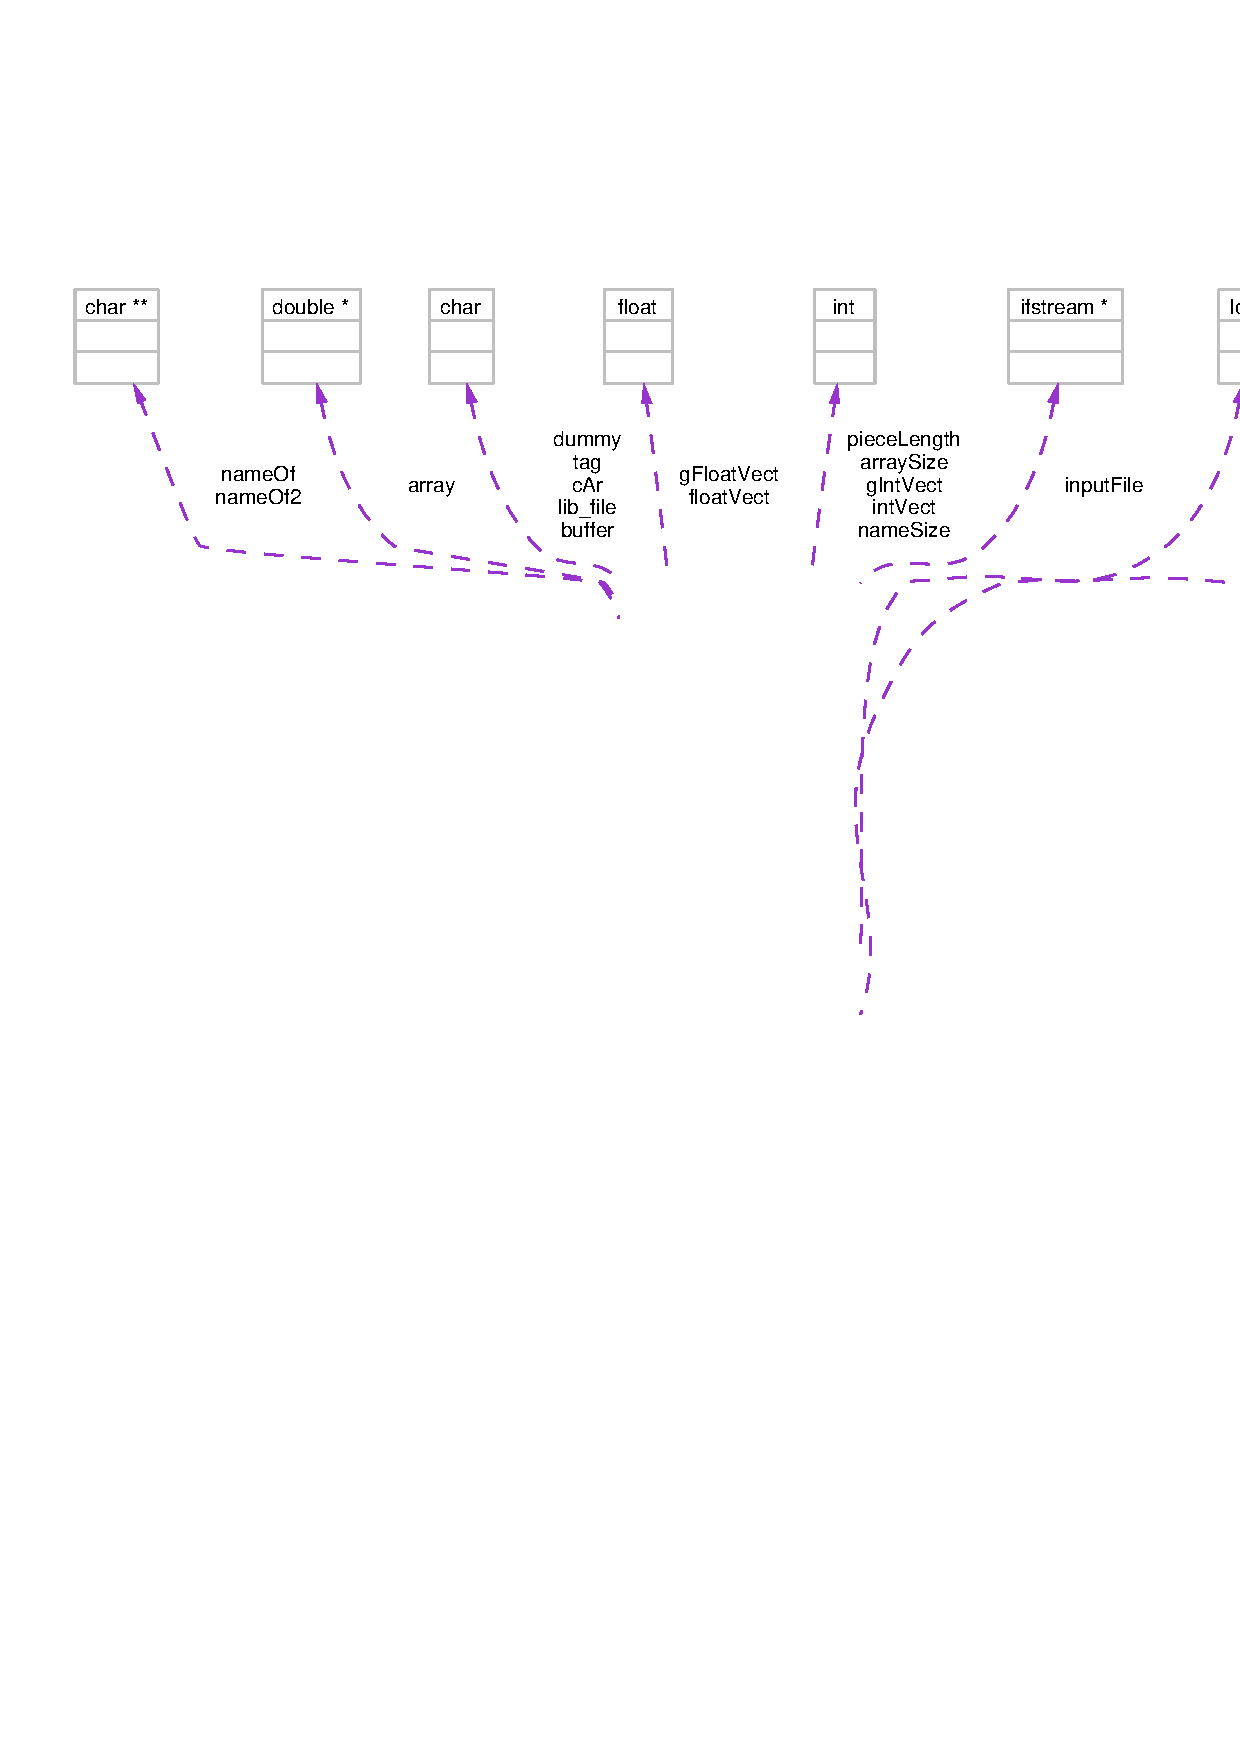
\includegraphics[width=373pt]{classDataIn__coll__graph}
\end{center}
\end{figure}
\subsection*{Public Member Functions}
\begin{CompactItemize}
\item 
{\bf Data\-In} (char $\ast$)
\item 
{\bf Data\-In} (int)
\item 
{\bf Data\-In} ()
\item 
{\bf $\sim$Data\-In} ()
\item 
void {\bf clear} ()
\item 
void {\bf Read\-Tags} (int size)
\item 
void {\bf Read\-Dummies} ()
\item 
void {\bf Read\-Char\-Array} ()
\item 
void {\bf Gen\-Ints} (int size)
\item 
void {\bf Gen\-Floats} (int size)
\item 
void {\bf Gen\-Chars} (int size)
\item 
void {\bf Read\-Ints} (int)
\item 
void {\bf Read\-Var\-Ints} (int, int)
\item 
void {\bf Read\-Floats} (int)
\item 
void {\bf Read\-FLong} (int)
\item 
void {\bf Read\-Array} (int)
\item 
void {\bf Read\-Chars} (int)
\item 
void {\bf Read\-Chars2} (int)
\item 
void {\bf open\-File} (char $\ast$)
\item 
void {\bf close\-File} ()
\item 
void {\bf rewind\-File} (long {\bf loc})
\item 
long {\bf file\-Loc} ()
\item 
void {\bf Remember\-File\-Loc} (int pos\-Num, char $\ast${\bf file\-Name}, long \&location)
\item 
void {\bf Skip} (int size)
\item 
void {\bf Read\-Buffer} ()
\end{CompactItemize}
\subsection*{Public Attributes}
\begin{CompactItemize}
\item 
int {\bf int\-Vect} [100]
\item 
int {\bf g\-Int\-Vect} [100]
\item 
float {\bf float\-Vect} [100]
\item 
float {\bf g\-Float\-Vect} [100]
\item 
long {\bf long\-Vect} [100]
\item 
char {\bf buffer} [80]
\item 
char {\bf dummy} [30]
\item 
char {\bf c\-Ar} [30]
\item 
char {\bf tag}
\item 
int {\bf array\-Size}
\item 
int {\bf name\-Size}
\item 
int {\bf piece\-Length}
\item 
long {\bf loc}
\item 
double $\ast$ {\bf array}
\item 
char $\ast$ {\bf file\-Name}
\item 
char {\bf lib\_\-file} [10]
\item 
char $\ast$$\ast$ {\bf name\-Of}
\item 
char $\ast$$\ast$ {\bf name\-Of2}
\end{CompactItemize}
\subsection*{Static Public Attributes}
\begin{CompactItemize}
\item 
ifstream $\ast$ {\bf input\-File} = NULL
\end{CompactItemize}
\subsection*{Private Member Functions}
\begin{CompactItemize}
\item 
void {\bf set\-File\-Name} (char $\ast$)
\end{CompactItemize}


\subsection{Constructor \& Destructor Documentation}
\index{DataIn@{Data\-In}!DataIn@{DataIn}}
\index{DataIn@{DataIn}!DataIn@{Data\-In}}
\subsubsection{\setlength{\rightskip}{0pt plus 5cm}Data\-In::Data\-In (char $\ast$)}\label{classDataIn_a0}




Definition at line 42 of file data\-In.cpp.

References array, file\-Name, input\-File, name\-Of, open\-File(), and set\-File\-Name().

Here is the call graph for this function:\begin{figure}[H]
\begin{center}
\leavevmode
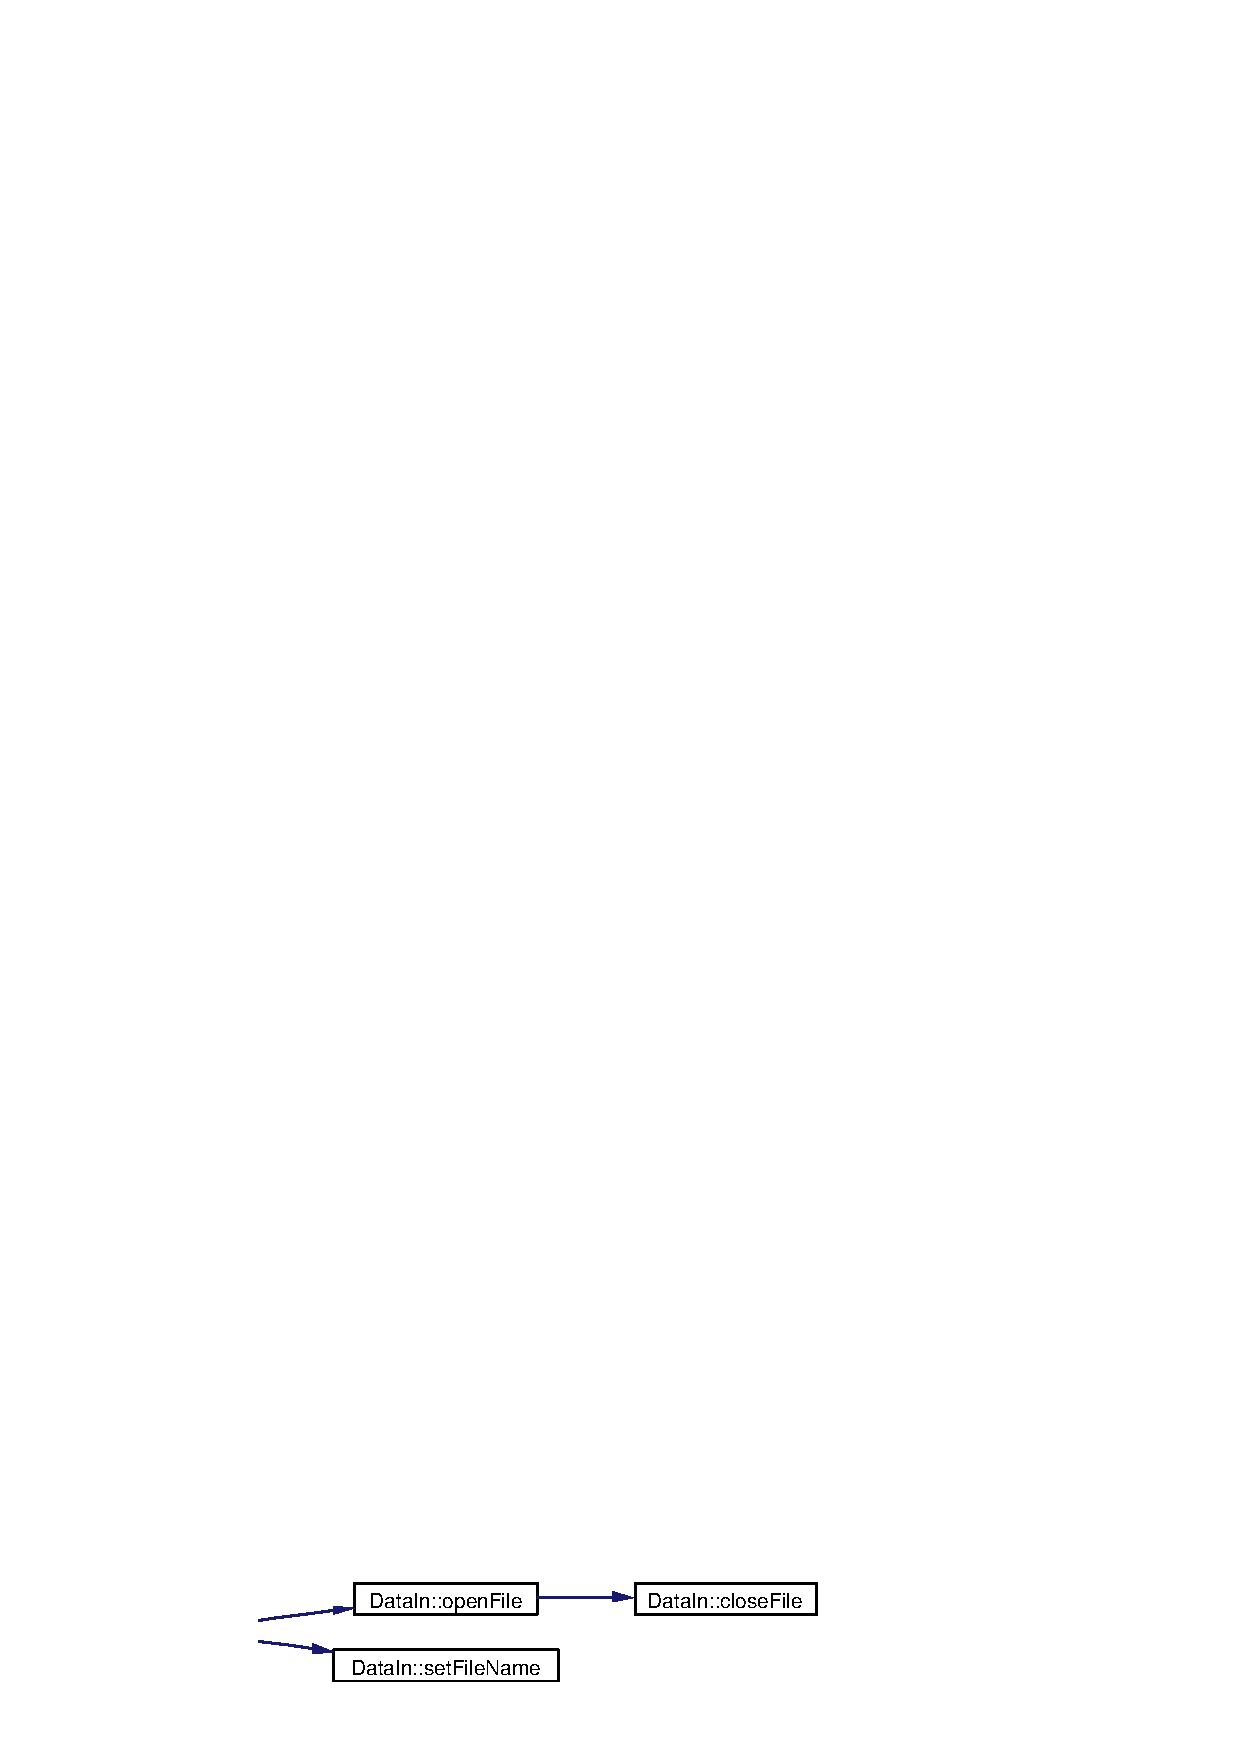
\includegraphics[width=200pt]{classDataIn_a0_cgraph}
\end{center}
\end{figure}
\index{DataIn@{Data\-In}!DataIn@{DataIn}}
\index{DataIn@{DataIn}!DataIn@{Data\-In}}
\subsubsection{\setlength{\rightskip}{0pt plus 5cm}Data\-In::Data\-In (int)}\label{classDataIn_a1}




Definition at line 61 of file data\-In.cpp.

References array, and name\-Of.\index{DataIn@{Data\-In}!DataIn@{DataIn}}
\index{DataIn@{DataIn}!DataIn@{Data\-In}}
\subsubsection{\setlength{\rightskip}{0pt plus 5cm}Data\-In::Data\-In ()}\label{classDataIn_a2}




Definition at line 73 of file data\-In.cpp.

References array, file\-Name, file\-Name, input\-File, name\-Of, and set\-File\-Name().

Here is the call graph for this function:\begin{figure}[H]
\begin{center}
\leavevmode
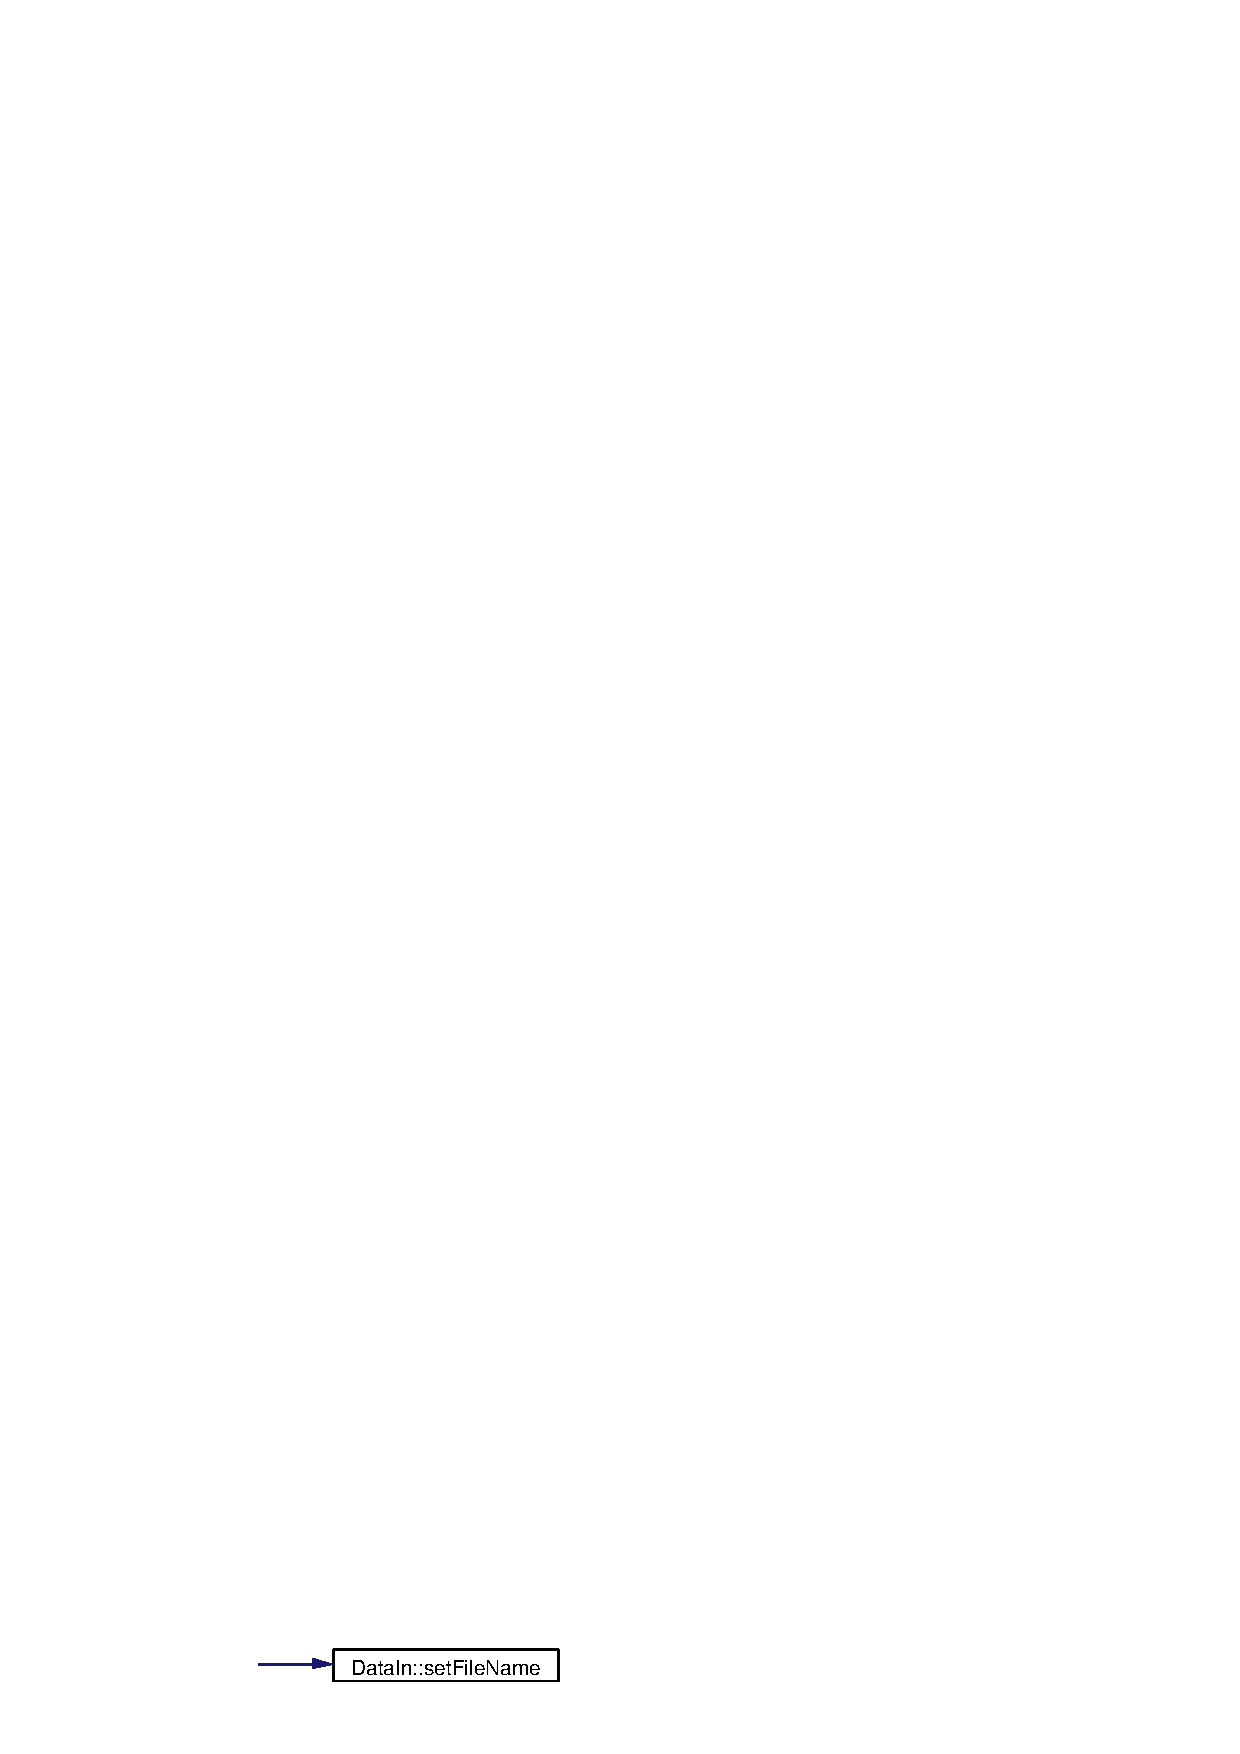
\includegraphics[width=138pt]{classDataIn_a2_cgraph}
\end{center}
\end{figure}
\index{DataIn@{Data\-In}!~DataIn@{$\sim$DataIn}}
\index{~DataIn@{$\sim$DataIn}!DataIn@{Data\-In}}
\subsubsection{\setlength{\rightskip}{0pt plus 5cm}Data\-In::$\sim${\bf Data\-In} ()}\label{classDataIn_a3}




Definition at line 94 of file data\-In.cpp.

References array, clear(), input\-File, loc, and name\-Of.

Here is the call graph for this function:\begin{figure}[H]
\begin{center}
\leavevmode
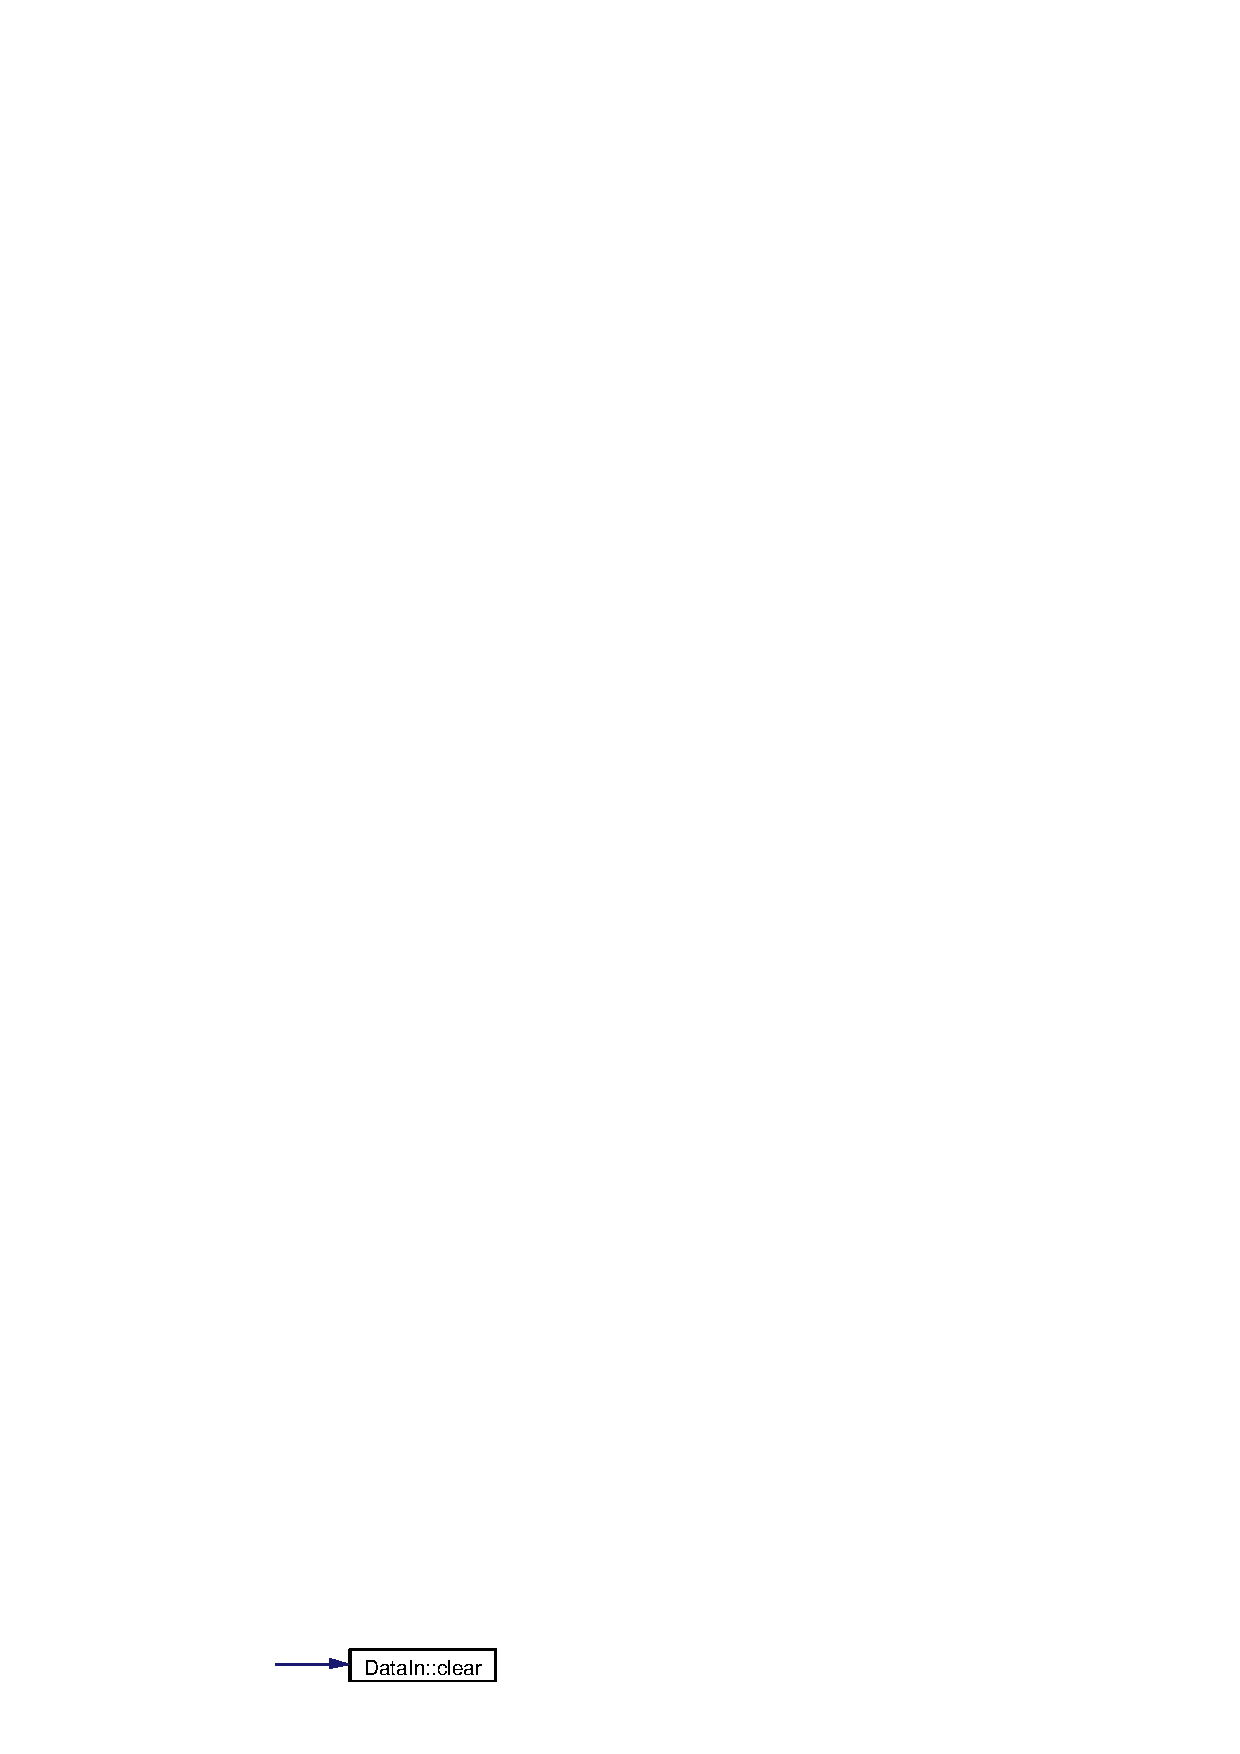
\includegraphics[width=123pt]{classDataIn_a3_cgraph}
\end{center}
\end{figure}


\subsection{Member Function Documentation}
\index{DataIn@{Data\-In}!clear@{clear}}
\index{clear@{clear}!DataIn@{Data\-In}}
\subsubsection{\setlength{\rightskip}{0pt plus 5cm}void Data\-In::clear ()}\label{classDataIn_a4}




Definition at line 108 of file data\-In.cpp.

References array, name\-Of, and name\-Size.

Referenced by $\sim$Data\-In().\index{DataIn@{Data\-In}!closeFile@{closeFile}}
\index{closeFile@{closeFile}!DataIn@{Data\-In}}
\subsubsection{\setlength{\rightskip}{0pt plus 5cm}void Data\-In::close\-File ()}\label{classDataIn_a19}




Definition at line 158 of file data\-In.cpp.

References input\-File.

Referenced by open\-File().\index{DataIn@{Data\-In}!fileLoc@{fileLoc}}
\index{fileLoc@{fileLoc}!DataIn@{Data\-In}}
\subsubsection{\setlength{\rightskip}{0pt plus 5cm}long Data\-In::file\-Loc ()}\label{classDataIn_a21}




Definition at line 181 of file data\-In.cpp.

References input\-File.

Referenced by Envelope\-Builder(), Event::Num\-Objs(), and Remember\-File\-Loc().\index{DataIn@{Data\-In}!GenChars@{GenChars}}
\index{GenChars@{GenChars}!DataIn@{Data\-In}}
\subsubsection{\setlength{\rightskip}{0pt plus 5cm}void Data\-In::Gen\-Chars (int {\em size})}\label{classDataIn_a10}




Definition at line 281 of file data\-In.cpp.

References input\-File, name\-Of, and name\-Size.

Referenced by Char\-Sequence().\index{DataIn@{Data\-In}!GenFloats@{GenFloats}}
\index{GenFloats@{GenFloats}!DataIn@{Data\-In}}
\subsubsection{\setlength{\rightskip}{0pt plus 5cm}void Data\-In::Gen\-Floats (int {\em size})}\label{classDataIn_a9}




Definition at line 245 of file data\-In.cpp.

References g\-Float\-Vect, and input\-File.

Referenced by Sequence().\index{DataIn@{Data\-In}!GenInts@{GenInts}}
\index{GenInts@{GenInts}!DataIn@{Data\-In}}
\subsubsection{\setlength{\rightskip}{0pt plus 5cm}void Data\-In::Gen\-Ints (int {\em size})}\label{classDataIn_a8}




Definition at line 263 of file data\-In.cpp.

References g\-Int\-Vect, and input\-File.

Referenced by Envelope\-Builder(), Patter::Get\-Patty(), and Patter::Init\-Pat().\index{DataIn@{Data\-In}!openFile@{openFile}}
\index{openFile@{openFile}!DataIn@{Data\-In}}
\subsubsection{\setlength{\rightskip}{0pt plus 5cm}void Data\-In::open\-File (char $\ast$)}\label{classDataIn_a18}




Definition at line 141 of file data\-In.cpp.

References close\-File(), file\-Name, and input\-File.

Referenced by Data\-In(), and Remember\-File\-Loc().

Here is the call graph for this function:\begin{figure}[H]
\begin{center}
\leavevmode
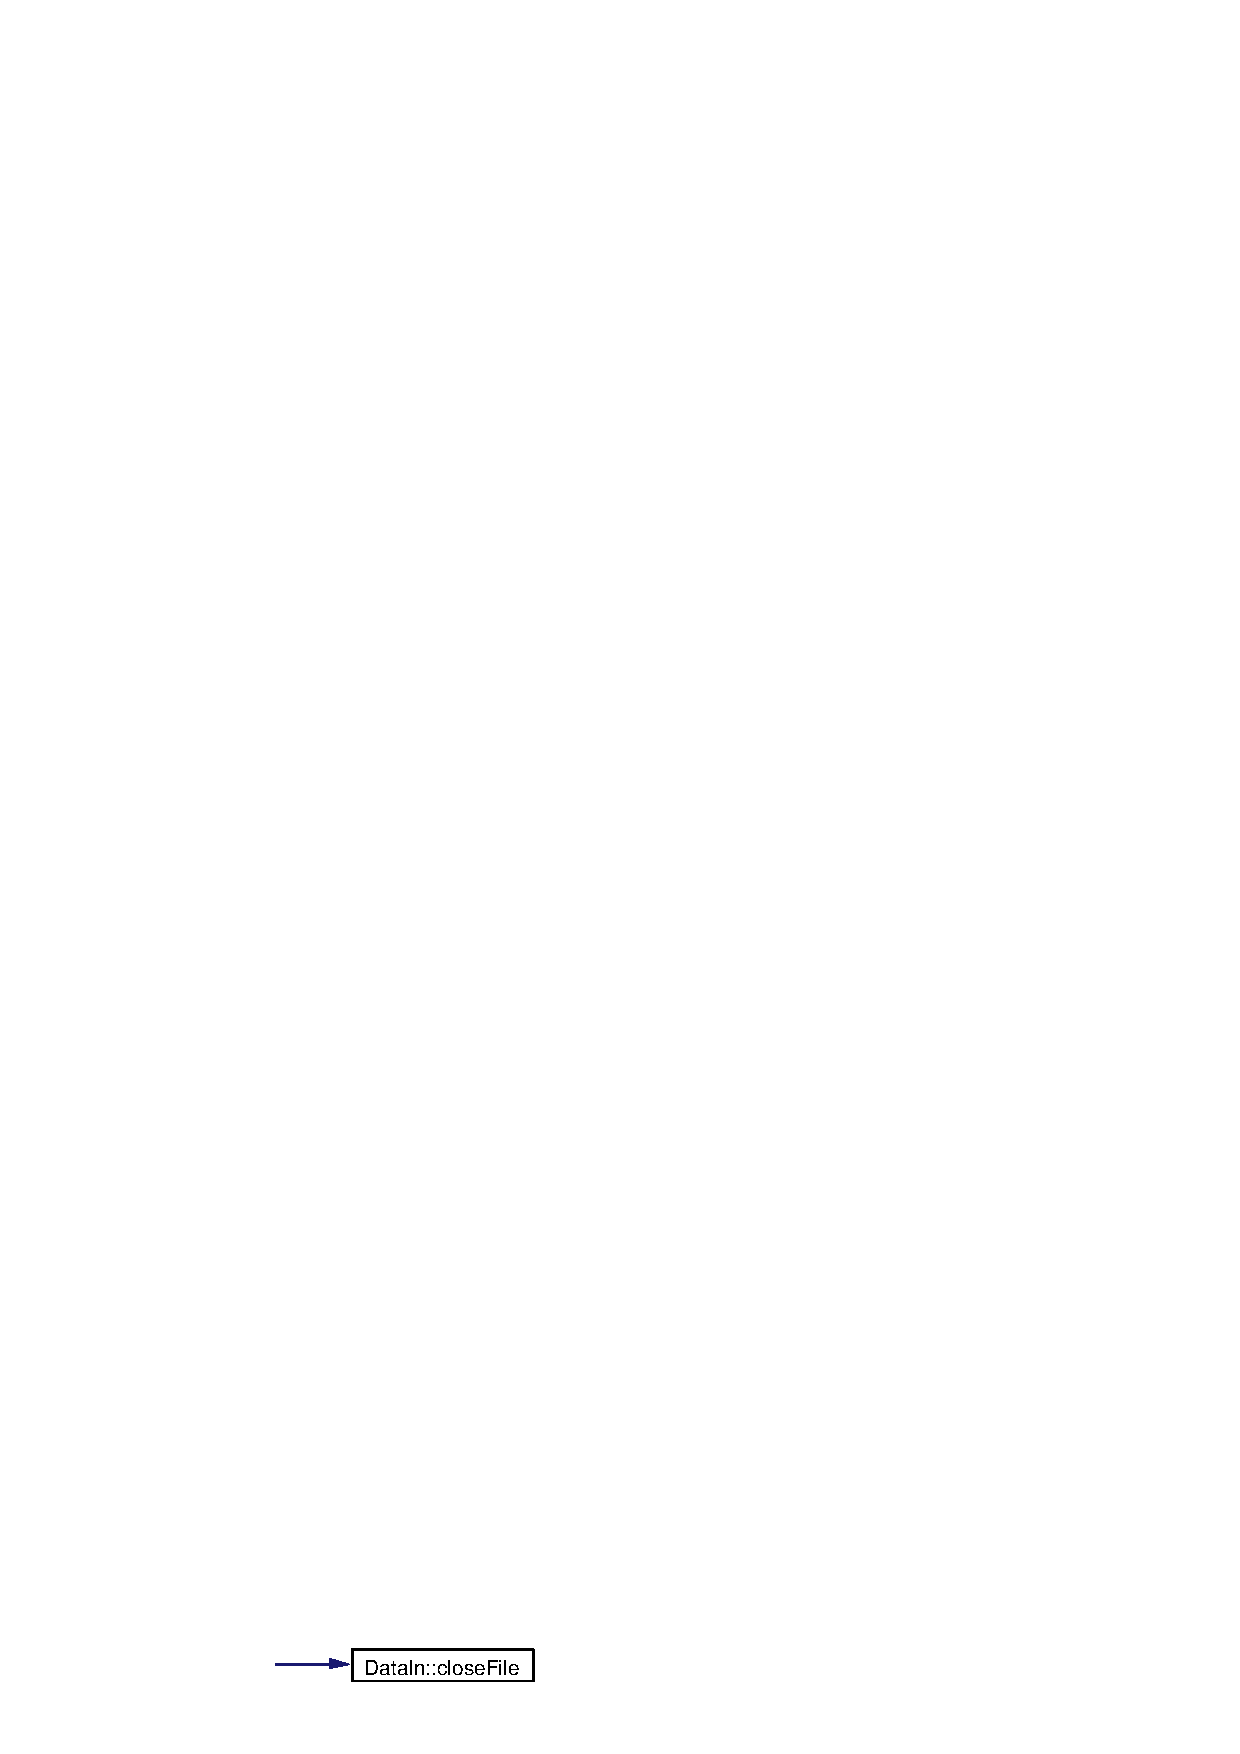
\includegraphics[width=132pt]{classDataIn_a18_cgraph}
\end{center}
\end{figure}
\index{DataIn@{Data\-In}!ReadArray@{ReadArray}}
\index{ReadArray@{ReadArray}!DataIn@{Data\-In}}
\subsubsection{\setlength{\rightskip}{0pt plus 5cm}void Data\-In::Read\-Array (int)}\label{classDataIn_a15}




Definition at line 385 of file data\-In.cpp.

References array, dummy, and input\-File.\index{DataIn@{Data\-In}!ReadBuffer@{ReadBuffer}}
\index{ReadBuffer@{ReadBuffer}!DataIn@{Data\-In}}
\subsubsection{\setlength{\rightskip}{0pt plus 5cm}void Data\-In::Read\-Buffer ()}\label{classDataIn_a24}




Definition at line 476 of file data\-In.cpp.

References buffer, and input\-File.

Referenced by Patter::Recorder().\index{DataIn@{Data\-In}!ReadCharArray@{ReadCharArray}}
\index{ReadCharArray@{ReadCharArray}!DataIn@{Data\-In}}
\subsubsection{\setlength{\rightskip}{0pt plus 5cm}void Data\-In::Read\-Char\-Array ()}\label{classDataIn_a7}




Definition at line 220 of file data\-In.cpp.

References c\-Ar, dummy, and input\-File.\index{DataIn@{Data\-In}!ReadChars@{ReadChars}}
\index{ReadChars@{ReadChars}!DataIn@{Data\-In}}
\subsubsection{\setlength{\rightskip}{0pt plus 5cm}void Data\-In::Read\-Chars (int)}\label{classDataIn_a16}




Definition at line 426 of file data\-In.cpp.

References dummy, input\-File, name\-Of, and name\-Size.

Referenced by Patter::Chooser(), Event::Copy\-Name(), Patter::Delivery(), Event::Duration\-Methods(), Patter::Expand(), Event::Num\-Objs(), Patter::Nursery(), Event::Points\-Probs(), and Event::Sweep3().\index{DataIn@{Data\-In}!ReadChars2@{ReadChars2}}
\index{ReadChars2@{ReadChars2}!DataIn@{Data\-In}}
\subsubsection{\setlength{\rightskip}{0pt plus 5cm}void Data\-In::Read\-Chars2 (int)}\label{classDataIn_a17}




Definition at line 444 of file data\-In.cpp.

References dummy, input\-File, name\-Of2, and name\-Size.\index{DataIn@{Data\-In}!ReadDummies@{ReadDummies}}
\index{ReadDummies@{ReadDummies}!DataIn@{Data\-In}}
\subsubsection{\setlength{\rightskip}{0pt plus 5cm}void Data\-In::Read\-Dummies ()}\label{classDataIn_a6}




Definition at line 208 of file data\-In.cpp.

References c\-Ar, and input\-File.

Referenced by Event::Copy\-Name(), Patter::Delivery(), Event::Duration\-Methods(), Patter::Get\-Patty(), Event::Layer\-Def(), Event::Num\-Objs(), Patter::Nursery(), and Event::Points\-Probs().\index{DataIn@{Data\-In}!ReadFloats@{ReadFloats}}
\index{ReadFloats@{ReadFloats}!DataIn@{Data\-In}}
\subsubsection{\setlength{\rightskip}{0pt plus 5cm}void Data\-In::Read\-Floats (int)}\label{classDataIn_a13}




Definition at line 342 of file data\-In.cpp.

References dummy, float\-Vect, and input\-File.

Referenced by Event::Points\-Probs().\index{DataIn@{Data\-In}!ReadFLong@{ReadFLong}}
\index{ReadFLong@{ReadFLong}!DataIn@{Data\-In}}
\subsubsection{\setlength{\rightskip}{0pt plus 5cm}void Data\-In::Read\-FLong (int)}\label{classDataIn_a14}




Definition at line 364 of file data\-In.cpp.

References dummy, input\-File, and long\-Vect.\index{DataIn@{Data\-In}!ReadInts@{ReadInts}}
\index{ReadInts@{ReadInts}!DataIn@{Data\-In}}
\subsubsection{\setlength{\rightskip}{0pt plus 5cm}void Data\-In::Read\-Ints (int)}\label{classDataIn_a11}




Definition at line 304 of file data\-In.cpp.

References dummy, input\-File, and int\-Vect.

Referenced by Char\-Sequence(), Event::Copy\-Name(), Patter::Equivalence(), Patter::Get\-Patty(), Patter::Init\-Pat(), Event::Layer\-Def(), Patter::Nursery(), Event::Points\-Probs(), Sequence(), and Event::Stimes().\index{DataIn@{Data\-In}!ReadTags@{ReadTags}}
\index{ReadTags@{ReadTags}!DataIn@{Data\-In}}
\subsubsection{\setlength{\rightskip}{0pt plus 5cm}void Data\-In::Read\-Tags (int {\em size})}\label{classDataIn_a5}




Definition at line 232 of file data\-In.cpp.

References input\-File, and tag.\index{DataIn@{Data\-In}!ReadVarInts@{ReadVarInts}}
\index{ReadVarInts@{ReadVarInts}!DataIn@{Data\-In}}
\subsubsection{\setlength{\rightskip}{0pt plus 5cm}void Data\-In::Read\-Var\-Ints (int, int)}\label{classDataIn_a12}




Definition at line 323 of file data\-In.cpp.

References dummy, input\-File, and int\-Vect.\index{DataIn@{Data\-In}!RememberFileLoc@{RememberFileLoc}}
\index{RememberFileLoc@{RememberFileLoc}!DataIn@{Data\-In}}
\subsubsection{\setlength{\rightskip}{0pt plus 5cm}void Data\-In::Remember\-File\-Loc (int {\em position\-Num}, char $\ast$ {\em file\-Name}, long \& {\em location})}\label{classDataIn_a22}


Remember\-File\-Location. 

Definition at line 191 of file data\-In.cpp.

References file\-Loc(), file\-Name, open\-File(), and rewind\-File().

Here is the call graph for this function:\begin{figure}[H]
\begin{center}
\leavevmode
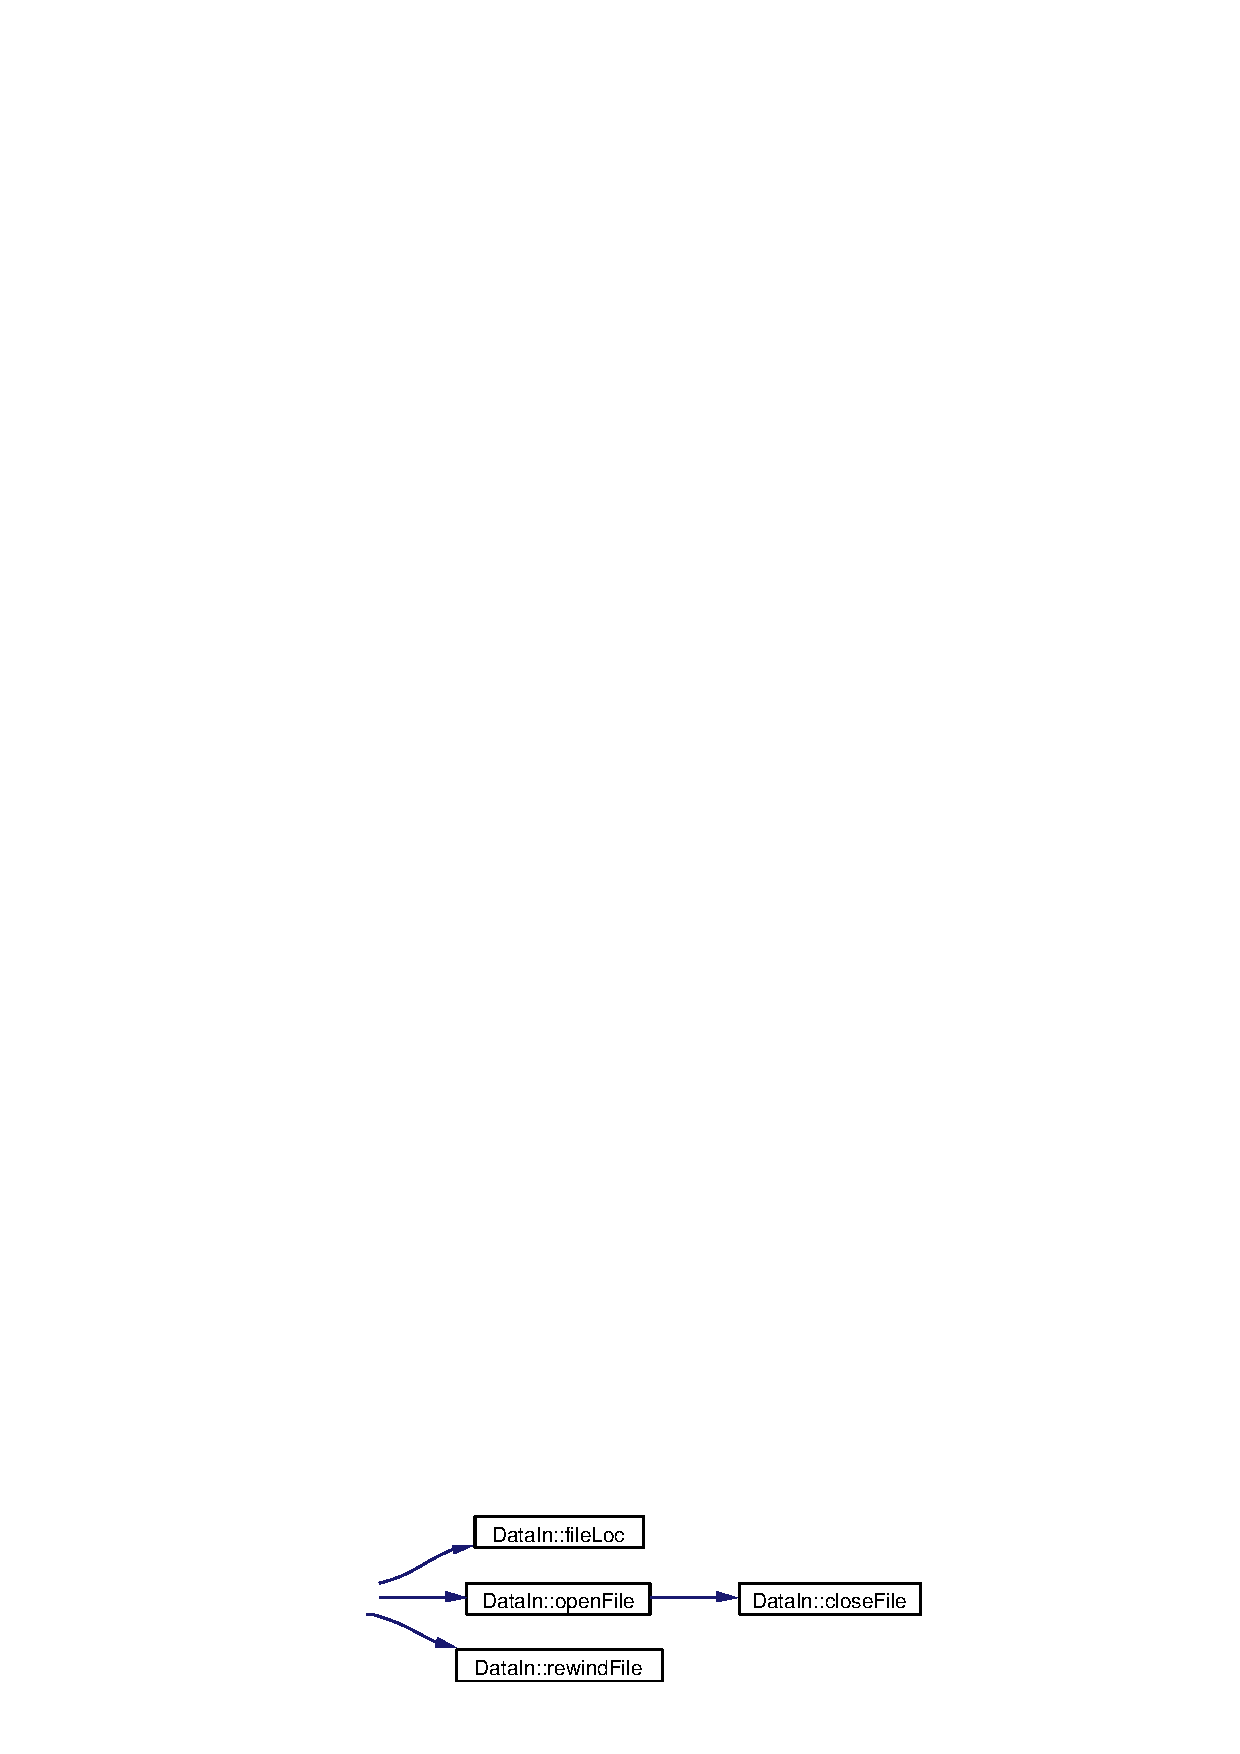
\includegraphics[width=225pt]{classDataIn_a22_cgraph}
\end{center}
\end{figure}
\index{DataIn@{Data\-In}!rewindFile@{rewindFile}}
\index{rewindFile@{rewindFile}!DataIn@{Data\-In}}
\subsubsection{\setlength{\rightskip}{0pt plus 5cm}void Data\-In::rewind\-File (long {\em loc})}\label{classDataIn_a20}




Definition at line 171 of file data\-In.cpp.

References input\-File.

Referenced by Envelope\-Builder(), Event::Num\-Objs(), Patter::Recorder(), and Remember\-File\-Loc().\index{DataIn@{Data\-In}!setFileName@{setFileName}}
\index{setFileName@{setFileName}!DataIn@{Data\-In}}
\subsubsection{\setlength{\rightskip}{0pt plus 5cm}void Data\-In::set\-File\-Name (char $\ast$)\hspace{0.3cm}{\tt  [private]}}\label{classDataIn_d0}




Definition at line 131 of file data\-In.cpp.

References file\-Name.

Referenced by Data\-In().\index{DataIn@{Data\-In}!Skip@{Skip}}
\index{Skip@{Skip}!DataIn@{Data\-In}}
\subsubsection{\setlength{\rightskip}{0pt plus 5cm}void Data\-In::Skip (int {\em size})}\label{classDataIn_a23}




Definition at line 462 of file data\-In.cpp.

References buffer, and input\-File.

Referenced by Patter::Get\-Patty().

\subsection{Member Data Documentation}
\index{DataIn@{Data\-In}!array@{array}}
\index{array@{array}!DataIn@{Data\-In}}
\subsubsection{\setlength{\rightskip}{0pt plus 5cm}double$\ast$ {\bf Data\-In::array}}\label{classDataIn_o13}




Definition at line 80 of file data\-In.h.

Referenced by clear(), Data\-In(), Read\-Array(), and $\sim$Data\-In().\index{DataIn@{Data\-In}!arraySize@{arraySize}}
\index{arraySize@{arraySize}!DataIn@{Data\-In}}
\subsubsection{\setlength{\rightskip}{0pt plus 5cm}int {\bf Data\-In::array\-Size}}\label{classDataIn_o9}




Definition at line 76 of file data\-In.h.\index{DataIn@{Data\-In}!buffer@{buffer}}
\index{buffer@{buffer}!DataIn@{Data\-In}}
\subsubsection{\setlength{\rightskip}{0pt plus 5cm}char {\bf Data\-In::buffer}[80]}\label{classDataIn_o5}




Definition at line 71 of file data\-In.h.

Referenced by Read\-Buffer(), Patter::Recorder(), and Skip().\index{DataIn@{Data\-In}!cAr@{cAr}}
\index{cAr@{cAr}!DataIn@{Data\-In}}
\subsubsection{\setlength{\rightskip}{0pt plus 5cm}char {\bf Data\-In::c\-Ar}[30]}\label{classDataIn_o7}




Definition at line 73 of file data\-In.h.

Referenced by Read\-Char\-Array(), and Read\-Dummies().\index{DataIn@{Data\-In}!dummy@{dummy}}
\index{dummy@{dummy}!DataIn@{Data\-In}}
\subsubsection{\setlength{\rightskip}{0pt plus 5cm}char {\bf Data\-In::dummy}[30]}\label{classDataIn_o6}




Definition at line 72 of file data\-In.h.

Referenced by Read\-Array(), Read\-Char\-Array(), Read\-Chars(), Read\-Chars2(), Read\-Floats(), Read\-FLong(), Read\-Ints(), and Read\-Var\-Ints().\index{DataIn@{Data\-In}!fileName@{fileName}}
\index{fileName@{fileName}!DataIn@{Data\-In}}
\subsubsection{\setlength{\rightskip}{0pt plus 5cm}char$\ast$ {\bf Data\-In::file\-Name}}\label{classDataIn_o14}




Definition at line 82 of file data\-In.h.

Referenced by Data\-In(), and set\-File\-Name().\index{DataIn@{Data\-In}!floatVect@{floatVect}}
\index{floatVect@{floatVect}!DataIn@{Data\-In}}
\subsubsection{\setlength{\rightskip}{0pt plus 5cm}float {\bf Data\-In::float\-Vect}[100]}\label{classDataIn_o2}




Definition at line 68 of file data\-In.h.

Referenced by Event::Points\-Probs(), and Read\-Floats().\index{DataIn@{Data\-In}!gFloatVect@{gFloatVect}}
\index{gFloatVect@{gFloatVect}!DataIn@{Data\-In}}
\subsubsection{\setlength{\rightskip}{0pt plus 5cm}float {\bf Data\-In::g\-Float\-Vect}[100]}\label{classDataIn_o3}




Definition at line 69 of file data\-In.h.

Referenced by Gen\-Floats(), and Sequence().\index{DataIn@{Data\-In}!gIntVect@{gIntVect}}
\index{gIntVect@{gIntVect}!DataIn@{Data\-In}}
\subsubsection{\setlength{\rightskip}{0pt plus 5cm}int {\bf Data\-In::g\-Int\-Vect}[100]}\label{classDataIn_o1}




Definition at line 67 of file data\-In.h.

Referenced by Envelope\-Builder(), Gen\-Ints(), Patter::Get\-Patty(), and Patter::Init\-Pat().\index{DataIn@{Data\-In}!inputFile@{inputFile}}
\index{inputFile@{inputFile}!DataIn@{Data\-In}}
\subsubsection{\setlength{\rightskip}{0pt plus 5cm}ifstream $\ast$ {\bf Data\-In::input\-File} = NULL\hspace{0.3cm}{\tt  [static]}}\label{classDataIn_s0}




Definition at line 34 of file data\-In.cpp.

Referenced by close\-File(), Data\-In(), file\-Loc(), Gen\-Chars(), Gen\-Floats(), Gen\-Ints(), open\-File(), Read\-Array(), Read\-Buffer(), Read\-Char\-Array(), Read\-Chars(), Read\-Chars2(), Read\-Dummies(), Read\-Floats(), Read\-FLong(), Read\-Ints(), Read\-Tags(), Read\-Var\-Ints(), rewind\-File(), Skip(), and $\sim$Data\-In().\index{DataIn@{Data\-In}!intVect@{intVect}}
\index{intVect@{intVect}!DataIn@{Data\-In}}
\subsubsection{\setlength{\rightskip}{0pt plus 5cm}int {\bf Data\-In::int\-Vect}[100]}\label{classDataIn_o0}




Definition at line 66 of file data\-In.h.

Referenced by Char\-Sequence(), Event::Copy\-Name(), Patter::Equivalence(), Patter::Get\-Patty(), Patter::Init\-Pat(), Event::Layer\-Def(), Patter::Nursery(), Event::Points\-Probs(), Read\-Ints(), Read\-Var\-Ints(), Sequence(), and Event::Stimes().\index{DataIn@{Data\-In}!lib_file@{lib\_\-file}}
\index{lib_file@{lib\_\-file}!DataIn@{Data\-In}}
\subsubsection{\setlength{\rightskip}{0pt plus 5cm}char {\bf Data\-In::lib\_\-file}[10]}\label{classDataIn_o15}




Definition at line 83 of file data\-In.h.\index{DataIn@{Data\-In}!loc@{loc}}
\index{loc@{loc}!DataIn@{Data\-In}}
\subsubsection{\setlength{\rightskip}{0pt plus 5cm}long {\bf Data\-In::loc}}\label{classDataIn_o12}




Definition at line 79 of file data\-In.h.

Referenced by $\sim$Data\-In().\index{DataIn@{Data\-In}!longVect@{longVect}}
\index{longVect@{longVect}!DataIn@{Data\-In}}
\subsubsection{\setlength{\rightskip}{0pt plus 5cm}long {\bf Data\-In::long\-Vect}[100]}\label{classDataIn_o4}




Definition at line 70 of file data\-In.h.

Referenced by Read\-FLong().\index{DataIn@{Data\-In}!nameOf@{nameOf}}
\index{nameOf@{nameOf}!DataIn@{Data\-In}}
\subsubsection{\setlength{\rightskip}{0pt plus 5cm}char$\ast$$\ast$ {\bf Data\-In::name\-Of}}\label{classDataIn_o16}




Definition at line 84 of file data\-In.h.

Referenced by Char\-Sequence(), Patter::Chooser(), clear(), Event::Copy\-Name(), Data\-In(), Patter::Delivery(), Event::Duration\-Methods(), Patter::Expand(), Gen\-Chars(), Event::Num\-Objs(), Patter::Nursery(), Event::Points\-Probs(), Read\-Chars(), Event::Sweep3(), and $\sim$Data\-In().\index{DataIn@{Data\-In}!nameOf2@{nameOf2}}
\index{nameOf2@{nameOf2}!DataIn@{Data\-In}}
\subsubsection{\setlength{\rightskip}{0pt plus 5cm}char$\ast$$\ast$ {\bf Data\-In::name\-Of2}}\label{classDataIn_o17}




Definition at line 85 of file data\-In.h.

Referenced by Read\-Chars2().\index{DataIn@{Data\-In}!nameSize@{nameSize}}
\index{nameSize@{nameSize}!DataIn@{Data\-In}}
\subsubsection{\setlength{\rightskip}{0pt plus 5cm}int {\bf Data\-In::name\-Size}}\label{classDataIn_o10}




Definition at line 77 of file data\-In.h.

Referenced by clear(), Gen\-Chars(), Read\-Chars(), and Read\-Chars2().\index{DataIn@{Data\-In}!pieceLength@{pieceLength}}
\index{pieceLength@{pieceLength}!DataIn@{Data\-In}}
\subsubsection{\setlength{\rightskip}{0pt plus 5cm}int {\bf Data\-In::piece\-Length}}\label{classDataIn_o11}




Definition at line 78 of file data\-In.h.\index{DataIn@{Data\-In}!tag@{tag}}
\index{tag@{tag}!DataIn@{Data\-In}}
\subsubsection{\setlength{\rightskip}{0pt plus 5cm}char {\bf Data\-In::tag}}\label{classDataIn_o8}




Definition at line 74 of file data\-In.h.

Referenced by Read\-Tags().

The documentation for this class was generated from the following files:\begin{CompactItemize}
\item 
{\bf data\-In.h}\item 
{\bf data\-In.cpp}\end{CompactItemize}
